\subsection{\large{\textit{cF}4-Cu (Inverse)}}\vspace{-0.1in}
Inverse Opal (FCC)


\begin{figure}[H]
\begin{minipage}{0.34\textwidth}\centering
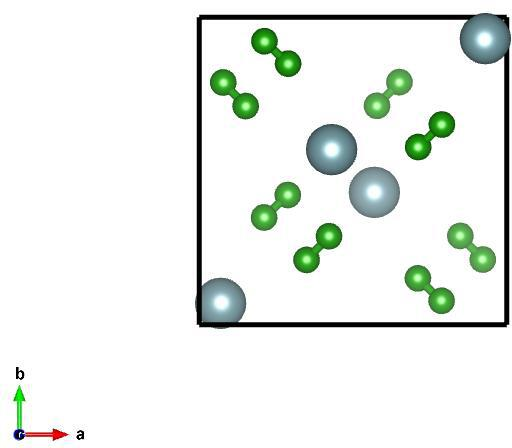
\includegraphics[width=0.9\linewidth,height=2in,keepaspectratio]{/Users/rosecers/work_folders/structures_for_photonics/reference/ref_inp/workspace/753d948145814bf0b1d0b01e05dcf303/final_images/analog_trim.jpg}\\
\small{Image of \textit{cF}4-Cu, generated by Vesta}
\end{minipage}\hfill
\begin{minipage}{0.65\textwidth}\raggedright
{\setlength{\mathindent}{0cm}
\begin{equation*}
\begin{split}&\boldsymbol{a_1} = 1/\sqrt{2}\ \hat{y} + 1/\sqrt{2}\ \hat{z}\\[-8pt]
&\boldsymbol{a_2} = 1/\sqrt{2}\ \hat{x} + 1/\sqrt{2}\ \hat{z}\\[-8pt]
&\boldsymbol{a_3} = 1/\sqrt{2}\ \hat{x} + 1/\sqrt{2}\ \hat{y}
\end{split}
\end{equation*}}

\textbf{Space Group:}	225\hspace{0.5in}\textbf{Point Group:}	$m\bar{3}m$\\
\textbf{Inorganic Crystallographic Database} \#43493\\
\textbf{Structure DOI: }\url{10.1063/1.1728392}

\textbf{Photonics DOI: }\url{10.1103/PhysRevLett.63.1950}
\end{minipage}\hfill
\end{figure}
\vspace{-0.25in}


\begin{figure}[H]
\begin{minipage}{0.9\textwidth}\centering
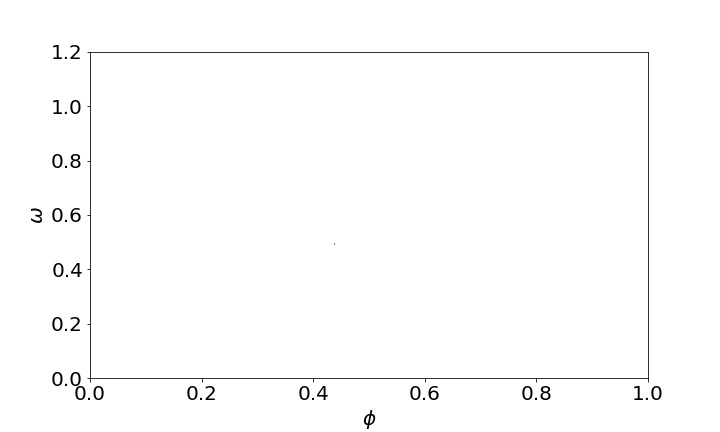
\includegraphics[width=0.9\linewidth,height=2.5in,keepaspectratio]{/Users/rosecers/work_folders/structures_for_photonics/reference/ref_inp/workspace/753d948145814bf0b1d0b01e05dcf303/final_images/gap_atlas.jpg}
\\
\end{minipage}\hfill\caption{Gap Atlas across filling fraction $\phi$ and frequency $\omega$}
\end{figure}


\begin{figure}[H]
\begin{minipage}{0.5\textwidth}\centering
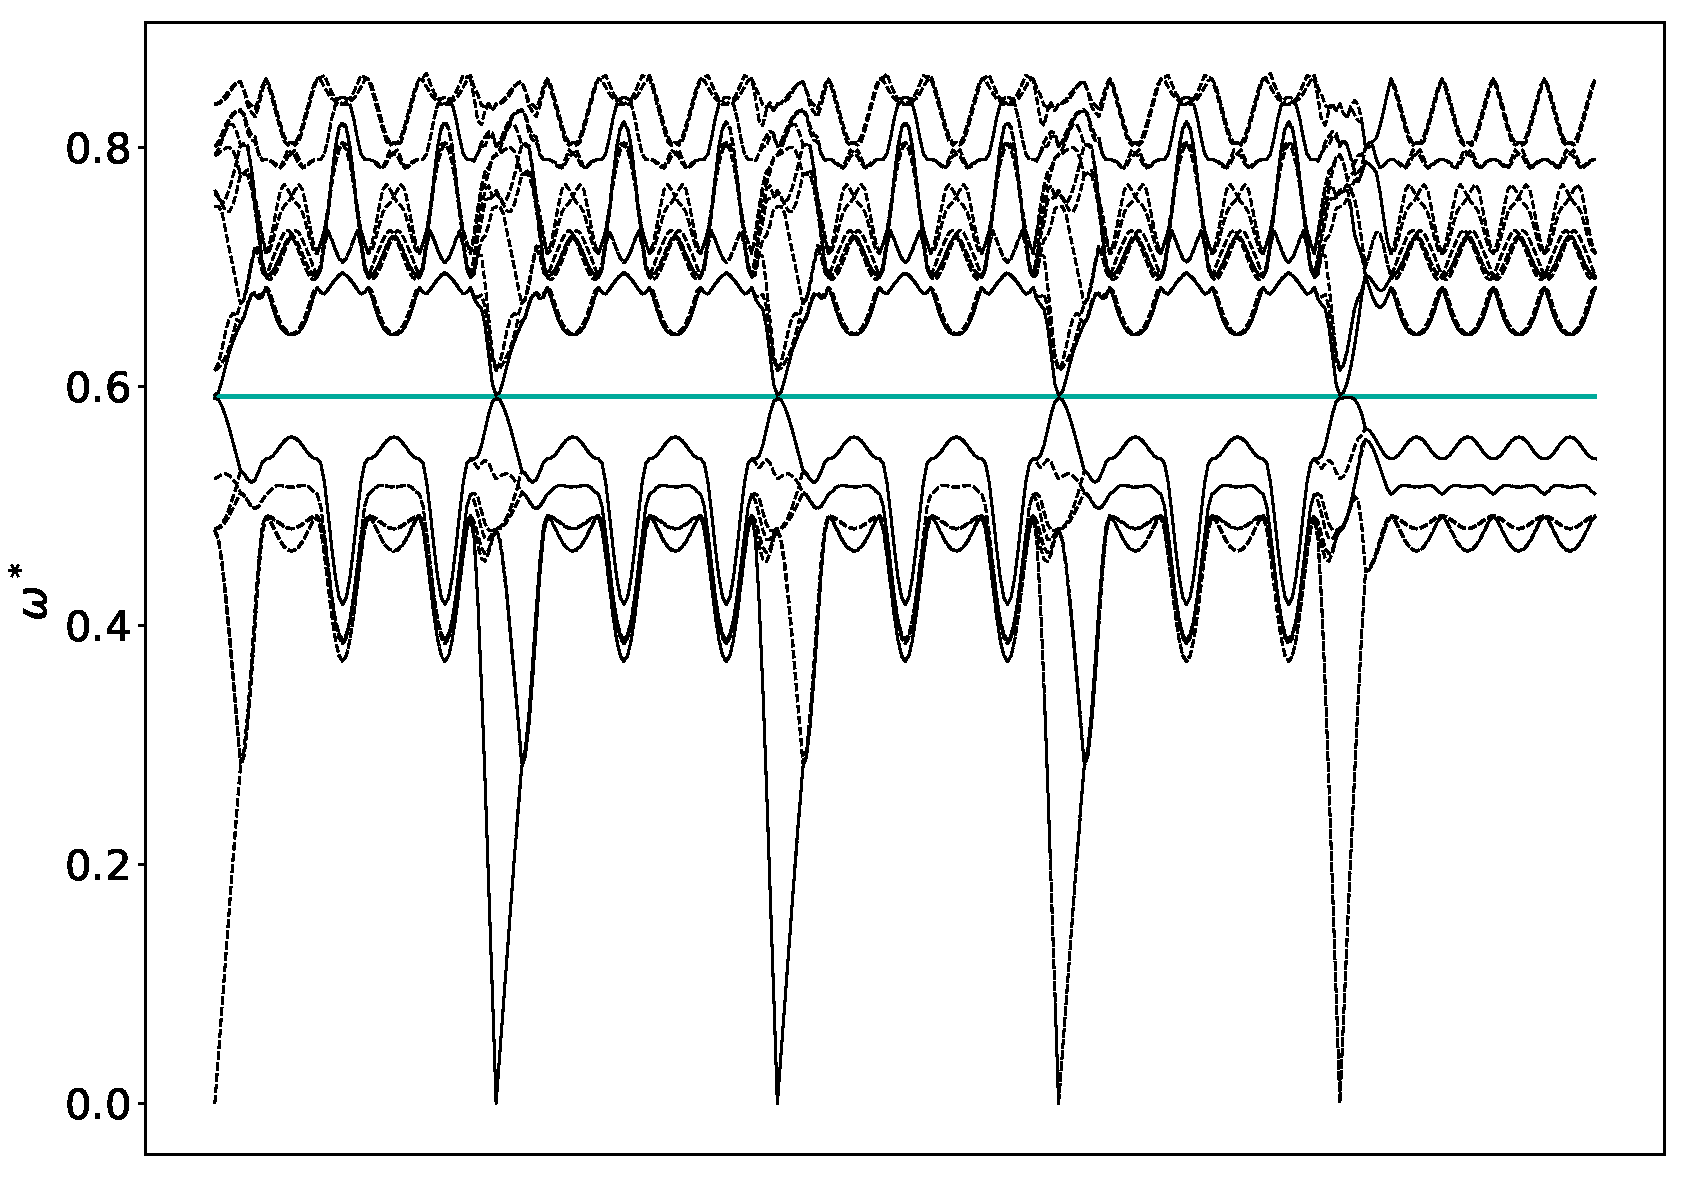
\includegraphics[width=0.9\linewidth,height=1.5in,keepaspectratio]{/Users/rosecers/work_folders/structures_for_photonics/reference/ref_inp/workspace/753d948145814bf0b1d0b01e05dcf303/./final_images/band_diagram_b=8.pdf}
\\Band Structure across 1st BZ
\end{minipage}\hfill
\begin{minipage}{0.48\textwidth}\centering
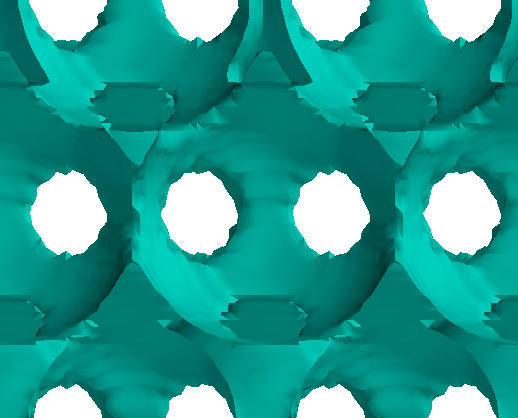
\includegraphics[width=0.9\linewidth,height=1.5in,keepaspectratio]{/Users/rosecers/work_folders/structures_for_photonics/reference/ref_inp/workspace/753d948145814bf0b1d0b01e05dcf303/final_images/cF4-Cu_r@gap_8-9.png}
\\View along $a_2$ 
\end{minipage}\hfill\caption{Band Structure and Isosurface of \textit{cF}4-Cu (Inverse) at radius = 0.51, filling fraction = 0.217, where the largest gap between bands 8 and 9 occurs with gap size 8.76\%.}

\end{figure}
\vspace{-0.25in}

